\section{Mô hình phân rã chức năng (BFD) và Kế hoạch thực hiện đồ án}

\subsection{Bảng phân rã chức năng nghiệp vụ (BFD)}
Hệ thống quản lý bán vé xem phim LumiCinema được phân rã thành 6 nhóm chức năng cấp 1 và các chức năng chi tiết cấp 2 như Bảng~\ref{tab:bfd}.

\begin{longtable}{|p{1.2cm}|p{4.3cm}|p{9.8cm}|}
\caption{Bảng phân rã chức năng nghiệp vụ (BFD) hệ thống LumiCinema} \label{tab:bfd} \\
\hline
\rowcolor{headerblue} \textbf{Mã} & \textbf{Chức năng cấp 1} & \textbf{Chức năng cấp 2} \\ \hline
\endhead
\textbf{1.0} & Quản lý tài khoản \& Xác thực & 1.1 Đăng ký tài khoản; 1.2 Đăng nhập / Đăng xuất; 1.3 Phân quyền theo vai trò (Khách hàng, Nhân viên, Admin). \\ \hline
\textbf{2.0} & Đặt vé \& Combo trực tuyến & 2.1 Xem danh sách phim \& suất chiếu; 2.2 Chọn ghế (sơ đồ 50 ghế A1--E10) \& loại vé; 2.3 Chọn combo bắp nước; 2.4 Áp dụng mã voucher; 2.5 Thanh toán qua ZaloPay/VNPay Gateway (kiểm tra số dư, nạp tiền, hoàn tiền tự động); 2.6 Gửi email xác nhận vé. \\ \hline
\textbf{3.0} & Quản lý vé khách hàng \& Đánh giá & 3.1 Xem danh sách vé đã mua; 3.2 Yêu cầu hủy vé ($\ge$ 2 giờ trước suất chiếu, nhận voucher 50\%); 3.3 Đánh giá phim (1--5 sao + bình luận). \\ \hline
\textbf{4.0} & Bán vé \& Soát vé tại quầy (POS) & 4.1 Bán vé \& combo tại quầy; 4.2 Tìm/gắn khách hàng theo SĐT/Email; 4.3 Thu tiền \& in vé; 4.4 Soát vé hợp lệ cho vào rạp; 4.5 Giao combo (chuyển trạng thái đã nhận). \\ \hline
\textbf{5.0} & Hủy vé, Bồi hoàn \& Xử lý sự cố & 5.1 Tra cứu thông tin vé tại quầy; 5.2 Hủy vé do khách (voucher 50\%); 5.3 Ép hủy vé sự cố rạp 1 bước (hoàn 100\% tiền mặt hoặc cấp voucher 100\% + gửi email); 5.4 Hủy toàn bộ suất chiếu sự cố \& giải phóng ghế. \\ \hline
\textbf{6.0} & Quản trị danh mục \& Báo cáo & 6.1 Quản lý Phim; 6.2 Quản lý Suất chiếu (khởi tạo 50 ghế); 6.3 Quản lý Combo \& tồn kho; 6.4 Quản lý Voucher; 6.5 Dashboard doanh thu (Streamgraph) \& Xuất báo cáo CSV. \\ \hline
\end{longtable}

\begin{figure}[H]
\centering
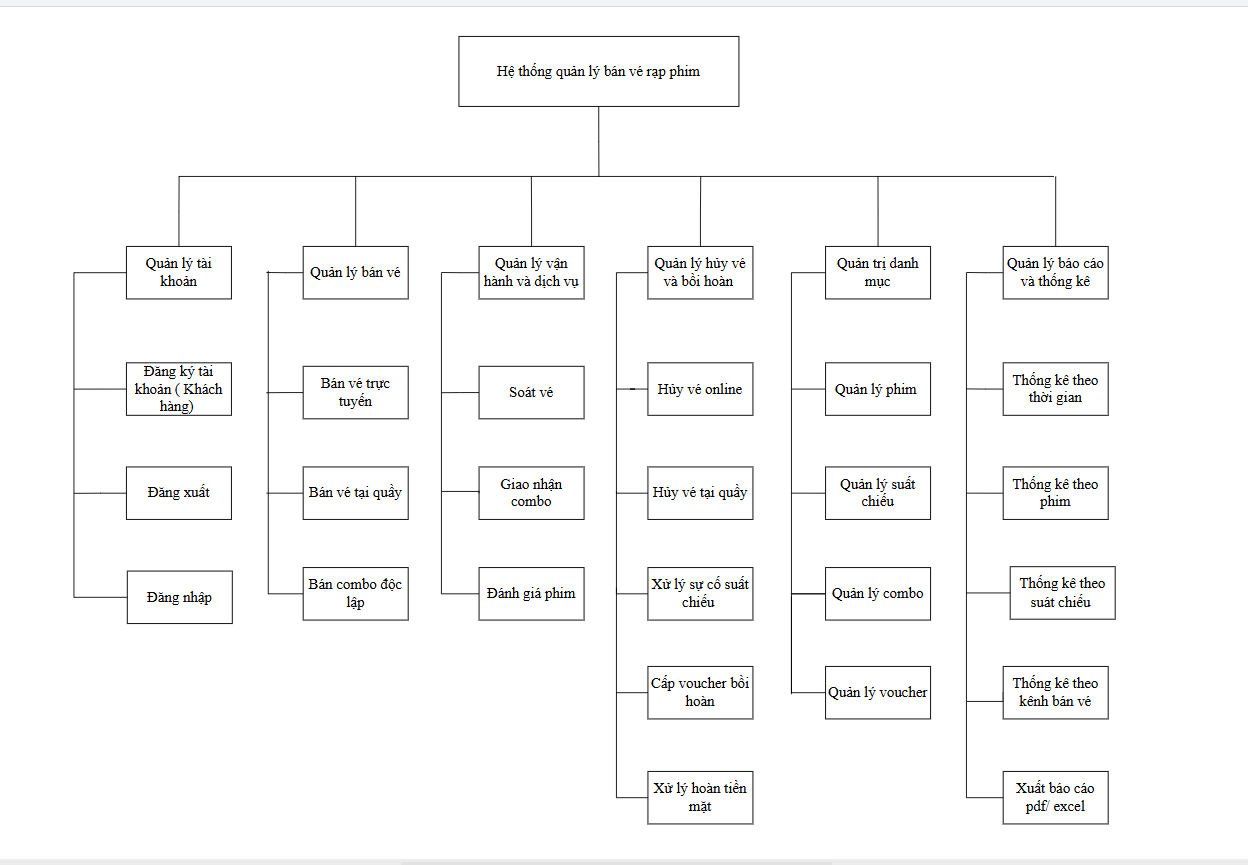
\includegraphics[width=\textwidth,height=0.80\textheight,keepaspectratio]{images/bfd/2.1_BFD_LumiCinema.png}
\caption{Sơ đồ phân rã chức năng (BFD) hệ thống LumiCinema}
\label{fig:bfd}
\end{figure}

\subsection{Kế hoạch thực hiện đồ án}
Đồ án được thực hiện trong 10 tuần với sự phân công rõ ràng cho 5 thành viên trong Nhóm 10 như Bảng~\ref{tab:plan}.

\begin{table}[H]
\centering
\caption{Kế hoạch thực hiện và phân công công việc Nhóm 10}
\label{tab:plan}
\renewcommand{\arraystretch}{1.25}
\begin{tabular}{|p{1.8cm}|p{5.5cm}|p{4.3cm}|p{3.5cm}|}
\hline
\rowcolor{headerblue} \textbf{Giai đoạn} & \textbf{Nội dung công việc} & \textbf{Phụ trách chính} & \textbf{Sản phẩm đầu ra} \\ \hline
Tuần 1--2 & Khảo sát yêu cầu, lập SRS, BFD, Use Case tổng quát và đặc tả Use Case & Mã Gia Vỹ \& cả nhóm & Tài liệu SRS, Sơ đồ Use Case \\ \hline
Tuần 3--4 & Thiết kế Sequence, Activity, State, Class Diagram, ERD và RDM & Hưng, Thắng, Bảo, Việt, Vỹ & Bộ sơ đồ UML \& CSDL chuẩn \\ \hline
Tuần 5--6 & Khởi tạo Next.js + Prisma + PostgreSQL, xây dựng xác thực, đặt vé online, POS & Hưng, Bảo, Vỹ & Module Auth, Booking, POS \\ \hline
Tuần 7--8 & Xây dựng hủy vé/bồi hoàn, đánh giá phim, ZaloPay/VNPay Gateway, Email SMTP, Dashboard & Thắng, Việt, Vỹ & Module Refund, Review, Admin \\ \hline
Tuần 9--10 & Kiểm thử tích hợp, đồng bộ 100\% tài liệu \& sơ đồ với code, đóng gói Docker \& hoàn thiện báo cáo & Cả nhóm & Bản chạy Docker + Báo cáo PDF \\ \hline
\end{tabular}
\end{table}
